\documentclass{article}
\usepackage[T1]{fontenc}
\usepackage{lmodern}
\usepackage[a3paper, margin=22mm]{geometry}
\usepackage{xcolor}
\usepackage{tikz}
\usepackage{array}

% Colours: background, accent shapes and text.
\definecolor{night}{HTML}{22223B}
\definecolor{violet}{HTML}{4A4E69}
\definecolor{blush}{HTML}{C9ADA7}
\definecolor{cream}{HTML}{F2E9E4}
\definecolor{gold}{HTML}{F4A259}

\renewcommand{\familydefault}{\sfdefault}
\pagestyle{empty}
\setlength{\parindent}{0pt}

\begin{document}
\color{cream}

% Background colour and decorative circles. Delete the circles for a plainer look.
\begin{tikzpicture}[remember picture, overlay]
  \fill[night] (current page.south west) rectangle (current page.north east);
  \fill[violet] ([xshift=-40mm, yshift=30mm]current page.north east) circle (120mm);
  \fill[gold] ([xshift=-40mm, yshift=30mm]current page.north east) circle (45mm);
  \draw[blush, line width=2pt] ([xshift=20mm, yshift=-30mm]current page.east) circle (55mm);
  \draw[blush, line width=2pt] ([xshift=20mm, yshift=-30mm]current page.east) circle (70mm);
\end{tikzpicture}

\vspace*{10mm}
{\fontsize{22}{26}\selectfont\bfseries\color{gold} PUBLIC SEMINAR SERIES \quad No.\ 7\par}
\vspace{40mm}

% Talk title and speaker.
{\fontsize{64}{70}\selectfont\bfseries How Cities\\ Remember\\ Their Rivers\par}
\vspace{16mm}
{\color{gold}\rule{60mm}{3pt}}
\vspace{12mm}

{\fontsize{30}{36}\selectfont\bfseries Dr. Imani Okoro\par}
\vspace{3mm}
{\fontsize{18}{24}\selectfont\color{blush} Urban historian, Department of Geography, Example University\par}
\vspace{18mm}

\begin{minipage}[t]{0.62\linewidth}
  \fontsize{15}{22}\selectfont
  Many cities buried their rivers under roads a century ago. Today some are digging them back up.
  This talk follows three rivers, in three cities, and asks what is gained, and lost, when a hidden stream sees daylight again.
\end{minipage}

\vfill

% Event details: edit date, time, place and booking.
\renewcommand{\arraystretch}{1.6}
\begin{minipage}[b]{0.72\linewidth}
  \fontsize{17}{22}\selectfont
  \begin{tabular}{@{}>{\bfseries\color{gold}}l@{\hspace{10mm}}l@{}}
    DATE & Thursday 8 October 2026 \\
    TIME & 18:00, doors open 17:30 \\
    PLACE & Lecture Theatre 2, Main Library \\
    ENTRY & Free, all welcome, no booking needed \\
  \end{tabular}
\end{minipage}\hfill
\begin{minipage}[b]{0.22\linewidth}
  \raggedleft
  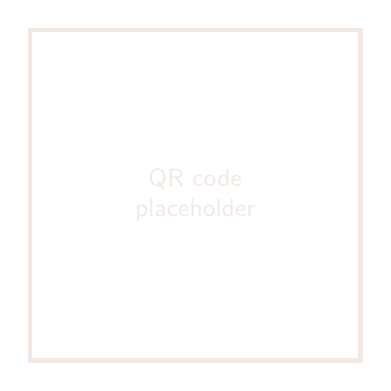
\begin{tikzpicture}
    \draw[cream, line width=1.5pt] (0,0) rectangle (42mm,42mm);
    \node[text width=36mm, align=center, font=\small, cream] at (21mm,21mm) {QR code\\placeholder};
  \end{tikzpicture}
\end{minipage}

\vspace{12mm}
{\color{violet}\rule{\linewidth}{1pt}}\par
\vspace{4mm}
{\small\color{blush} Organised by the Example City Heritage Society \hfill heritage@example.org\par}

\end{document}
